\documentclass[12pt,a4paper]{article}
\usepackage{amsmath,amssymb,fullpage,graphicx}
\let\hat\widehat
\let\tilde\widetilde

\usepackage{amssymb}
\usepackage{amsmath}
\usepackage{epsfig, graphics}
\usepackage{latexsym}
\usepackage{fullpage}
\usepackage{bm}
\usepackage[parfill]{parskip}
\usepackage{subfigure}
% TODO : Fil your personal package here if needed

%%%% new version of enumerate with less spacing
\newenvironment{enum}{
\begin{enumerate}
  \setlength{\itemsep}{1pt}
  \setlength{\parskip}{0pt}
  \setlength{\parsep}{0pt}
}{\end{enumerate}}

% TODO : fill your custom commands here if needed
\newcommand{\Ab}{\bm{A}}

\begin{document}

% TODO : Fill your personal information here
\begin{center}
    {\bf\large Homework 1} \\
    {\bf\large M1522.001300 Probabilistic Graphical Models (2016 Fall)} \\
    2016-21188 Byeongchang Kim \\
    % Due: September 22 Thursday 11:59PM \\
    Date: September 22 Thursday
\end{center}

Fill anything you want to say about your homework.

% TODO : Fill your answers
%%%%%%%%%%%%%%%%%%%%%%%%%%%%%%%%%%%%%%%%%%%%%%
% Q1
%%%%%%%%%%%%%%%%%%%%%%%%%%%%%%%%%%%%%%%%%%%%%%
\section{Conditional Independence Properties [15 points]}

Fill your answers.

You can insert your figure by using \verb|\begin{figure}|.
You can refer your figure by using \verb|\ref{fig:example_figure}|.

\begin{figure}[!h]
    \begin{center}
        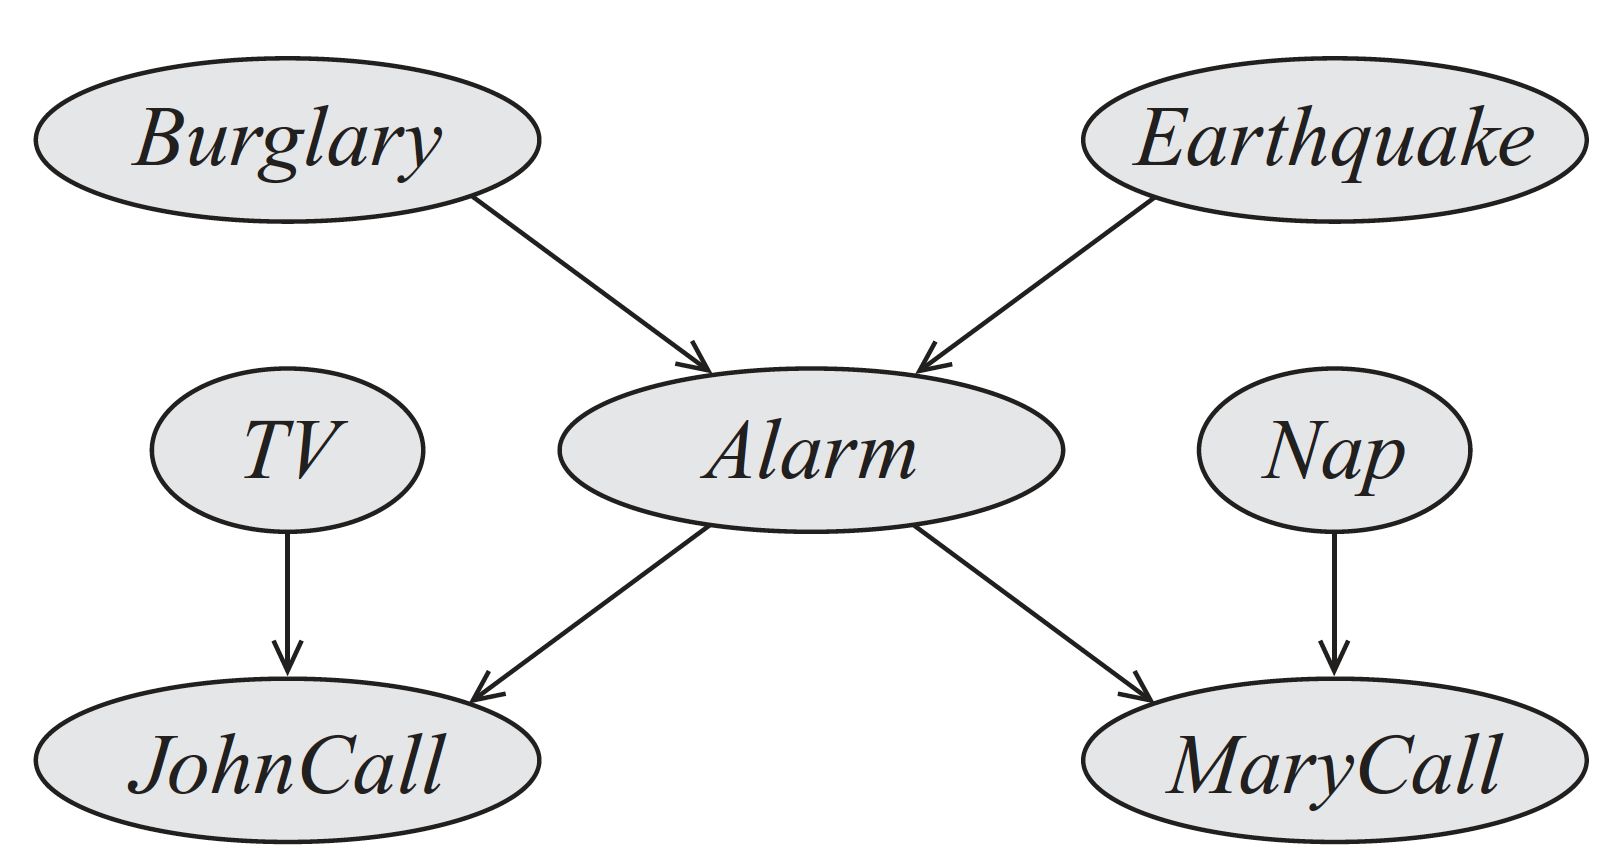
\includegraphics[width=0.7\textwidth]{assets/fig1.png}
        \caption{Example Figure}
        \label{fig:example_figure}
    \end{center}
\end{figure}

You can enumerate subquestions like this.

\begin{enumerate}
    \item Enumerate item 1.
    \item Enumerate item 2.
    \item Enumerate item 3.
\end{enumerate}

You can write your equations by using \verb|\begin{aligned}|.
We highly recommend you to use \verb|\newcommand| to simplify your equation in \LaTeX.

$$
\begin{aligned}
    \Ab &= 12 \\
    \alpha_{12}^{35} &= 1234 \\
    \beta_1 &= 10
\end{aligned}
$$

You can cite your reference by using \verb|\cite{reference_name}|.
For example, cite Koller's PGM book \cite{KollerPGM} like this.


%%%%%%%%%%%%%%%%%%%%%%%%%%%%%%%%%%%%%%%%%%%%%%
% Q2
%%%%%%%%%%%%%%%%%%%%%%%%%%%%%%%%%%%%%%%%%%%%%%
\section{Variance [5 points]}

Fill your answers.

% Bibtex
\bibliography{writeup}
\bibliographystyle{plain}

\end{document}
